\documentclass[11pt]{article}
\usepackage[margin=0.95in]{geometry}
\usepackage{amsmath,amssymb,booktabs,tikz,hyperref}
\hypersetup{hidelinks,pdfauthor={Rohan Arun},pdftitle={Minimum numbers of convex polygons on twelve and thirteen points}}
\setlength{\parindent}{1.05em}\setlength{\parskip}{2pt}
\setlength{\abovedisplayskip}{7pt}\setlength{\belowdisplayskip}{7pt}
\pagestyle{plain}
\begin{document}
\begin{center}
{\LARGE\bfseries Minimum numbers of convex polygons\\[3pt] on twelve and thirteen points}\\[12pt]
{\large Rohan Arun}\\[2pt] Super Powers AI\\[4pt]
{\small Research draft, November 20, 2026}
\end{center}
\begin{abstract}
Among twelve points in the plane with no three collinear, the least possible number of convex polygons is 408. Among thirteen points it is 570. Exactly five thirteen-point order types attain equality up to reflection and relabeling. We obtain the lower bounds by enumerating orientation signs along a chain of point deletions and certifying the nonrealizability of the remaining exceptions by inequalities between triangle areas. Integer coordinates certify attainment. The same search independently recovers Savova's ten- and eleven-point values.
\end{abstract}
\section{The finite problem}
For a finite planar point set $S$ with no three collinear, let $C(S)$ count the subsets of at least three points in convex position. All vertices of a counted subset must lie on its hull. Other points of $S$ may lie inside that hull. Write $f(n)=\min_{|S|=n}C(S)$. Erd\H{o}s and Hammer asked how small this number could be. Erd\H{o}s also asked whether $\log f(n)/(\log n)^2$ has a limit~\cite{erdos}. The latter question remains open.

\noindent\textbf{Theorem.} $f(12)=408$ and $f(13)=570$. At thirteen points, exactly five order types attain the minimum, up to permutations and simultaneous reversal of orientations. Their profiles appear in Table~1.

Savova~\cite{savova} counted all nonempty subsets in convex position. She obtained the ten-point minimum by scanning the Graz order-type database~\cite{graz} and the eleven-point minimum by a separate extension argument. Her convention includes $n+\binom n2$ additional subsets. Consequently her values 244 and 349 give $f(10)=189$ and $f(11)=283$. Conversely, the new values in her convention are 486 and 661. An earlier public computation by the Erd\H{o}s Problem a Day project tabulated the polygon convention through nine points~\cite{prior}.

\begin{center}
\begin{tabular}{r r r r r r l}\toprule
$n$ & Triangles & Quadrilaterals & Pentagons & Hexagons & Total & Scope\\\midrule
10 & 120 & 66 & 3 & 0 & 189 & known value\\
11 & 165 & 108 & 10 & 0 & 283 & known value\\
12 & 220 & 165 & 22 & 1 & 408 & one witness\\
13 & 286 & 241 & 41 & 2 & 570 & one type\\
13 & 286 & 247 & 35 & 2 & 570 & four types\\\bottomrule
\end{tabular}\par\smallskip
{\small Table 1. Counts in explicit minimizers. All displayed sets have no convex subset of size seven.}
\end{center}

\newpage
\section{An exhaustive lower-bound search}
Let $Q$ and $P$ be the convex quadrilateral and pentagon counts. Every triple contributes one triangle. Consequently a twelve-point set with $C\le407$ has $Q+P\le187$. To include all thirteen-point minimizers as well as every possible improvement on 570, we impose $Q+P\le284$ at thirteen points.

\paragraph{Deletion.} Suppose an $m$-point set satisfies $A Q+B P\le T$ with nonnegative weights. Write $Q_i,P_i$ for the counts after deletion of point $i$. Every quadrilateral survives $m-4$ deletions and every pentagon survives $m-5$. Averaging over $i$ gives a deletion satisfying
\[
 A(m-5)Q_i+B(m-4)P_i
 \ \le\ \left\lfloor \frac{(m-4)(m-5)T}{m}\right\rfloor.
\]
Divide the coefficients by their greatest common divisor, rounding the new bound down. At $m=5$, use $\sum_i Q_i=Q$ and $AQ\le T$. Iteration produces a nested chain down to a triangle for every candidate point set.

\paragraph{Reversing the chain.} Store the sign of the oriented area $[ijk]=\det(x_j-x_i,x_k-x_i)$ for every ordered triple, using alternation. To add $x$ to an old set, consider one old point $i$. The lines $ij$ cut the directions about $i$ into open angular intervals. Beside the ray $ij$, the signs of $[ikx]$ for $k\ne i,j$ are those of $[ikj]$, and $[ijx]$ can have either sign. Include the opposite directions as well. Taking all $j$ covers every interval, since each interval borders a ray. Choose one sign row for every $i$ and require $[ijx]$ and $[jix]$ to have opposite signs. These separate choices can produce spurious patterns. They cover every geometric extension of every realization of the old signs.

\paragraph{Counting and equivalence.} For four points $a,b,c,d$, the coefficients of their affine dependence have signs
\[
 \operatorname{sgn}\bigl([bcd],-[acd],[abd],-[abc]\bigr)
\]
componentwise. The coefficients sum to zero. Four equal signs are impossible. Two of each sign correspond to a convex quadrilateral, and a 1--3 split puts one point inside the other three. A set of at least five points is in convex position if and only if all its four-point subsets are. Indeed, a selected point in the convex hull of the others lies in the triangle of three of them by planar Carath\'eodory. This gives the total count using integer signs alone.

We discard patterns above their deletion bound and keep one copy of each signature obtained by relabeling and reflection. For a realizable type, try each hull vertex as first label, read the other vertices in angular order in either direction, and allow simultaneous reversal of all triple signs. An order type records the orientation of every labeled triple. The least resulting bit string is invariant under relabeling and reflection. At a hull vertex all other points occupy an open half-plane, so the angular order is determined by the signs. Every key, including for a spurious pattern, is a relabeling with optional sign reversal. A collision therefore never removes a distinct realizable order type. Induction up the deletion chain shows that the final list contains every realizable candidate.

\newpage
\section{Exclusions and attainment}
The final searches give the following numbers of distinct signatures. The middle column includes all signatures passing the indicated $Q+P$ bound. The last column also applies the full polygon count.
\begin{center}
\begin{tabular}{r r r l}\toprule
$n$ & $Q+P$ bound & Signatures & Full-count candidates\\\midrule
10 & 68 & 0 & none with $C\le188$\\
11 & 117 & 0 & none with $C\le282$\\
12 & 187 & 92 & six with $C=407$, none below\\
13 & 284 & 625 & one with $C=569$, ten with $C=570$, none below 569\\\bottomrule
\end{tabular}
\end{center}
For each of the six 407-candidates and for the unique 569-candidate we give a biquadratic final polynomial, using the method of Bokowski and Richter~\cite{br}. Write
\[
 U_0=[abc][ade],\qquad U_1=[abd][ace],\qquad U_2=[abe][acd].
\]
Expansion gives $U_0-U_1+U_2=0$. When one of the three signed terms has the opposite sign to the other two, its magnitude exceeds each of theirs. A certificate lists such strict inequalities, with positive multiplicities, for which each area factor occurs equally often on both sides. Multiplying them would make a positive number exceed itself. Hence the specified signature has no real realization. At twelve points each certificate needs ten or eleven distinct comparisons. At thirteen points, nine suffice to exclude the 569-candidate. Five of the ten 570-candidates have certificates of the same form.

The other five have integer-coordinate realizations. For each, we checked every triple sign and computed the hull of every subset, retaining subsets whose hull contains all selected points as vertices. The five canonical signatures differ. This proves the two lower bounds, attainment and the thirteen-point classification. \hfill$\square$

\begin{center}
\begin{minipage}{0.29\linewidth}\centering
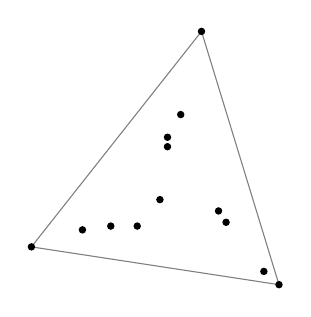
\begin{tikzpicture}[x=.024cm,y=.024cm]
\draw[gray] (0,20)--(131,0)--(90,134)--cycle;
\foreach \x/\y in {27/29,131/0,68/45,103/33,0/20,79/90,99/39,123/7,42/31,90/134,72/78,72/73,56/31}
 \fill (\x,\y) circle[radius=1.35pt];
\end{tikzpicture}
\end{minipage}\hfill
\begin{minipage}{0.65\linewidth}\small
\textbf{Figure 1.} One of the five minimizing configurations. Its thirteen points determine 286 triangles, 241 quadrilaterals, 41 pentagons and two hexagons. The outline is the convex hull of the entire configuration.
\end{minipage}
\end{center}
\paragraph{Reproducibility.} Extract the companion archive and run \texttt{python3 replay.py} with a C++17 compiler installed. The program regenerates the candidate lists, checks the signs and cancellation in the exclusion certificates, and verifies the witnesses. The search for the certificates is unnecessary for replay. The separate Lean archive checks specific witnesses and determinant exclusions. Exhaustiveness uses the argument on page~2 and the enumeration program.

\newpage
\section*{A nine-comparison certificate}
Here is the certificate for the only thirteen-point signature giving 569 polygons. Each row specifies the five labels $(a,b,c,d,e)$ and a strict inequality $|U_s|>|U_t|$, with the $U_j$ defined above. All multiplicities are one. The labels start at zero and correspond to the candidate's stored triple signs.
\begin{center}
\begin{tabular}{rrrrr@{\hspace{1.8em}}cc}\toprule
$a$&$b$&$c$&$d$&$e$&$s$&$t$\\\midrule
0&2&3&6&9&1&0\\2&0&3&6&12&0&1\\3&2&7&8&12&2&1\\
7&3&8&9&12&2&0\\8&2&3&9&10&0&2\\9&0&3&7&8&1&0\\
9&0&6&7&12&0&1\\10&2&8&9&12&0&2\\12&2&6&9&10&2&0\\\bottomrule
\end{tabular}
\end{center}
For example, the first row asserts
\[
 |[0,2,6][0,3,9]|>|[0,2,3][0,6,9]|.
\]
The factor $|[0,2,6]|$ occurs on the right of the second row as $|[2,0,6]|$. The reader can similarly pair every factor. Here are the signs of the candidate's triples, ordered lexicographically with the indices within each triple increasing. A one denotes positive orientation. Reading across the lines gives all 286 signs.

{\small\begin{verbatim}
0000000000000000000000000000000000000000000000000000000000
0000000001000011111000111110000111101111111111111111111111
1111110001111100001111011111111111111111111111111100001011
0111111111111111111011011111011111111111111111111100111111
111101000100000000001000100000000010110001110001101110
\end{verbatim}}
\paragraph{Computational assistance.} OpenAI Codex assisted with mathematical derivations, code, certificate generation, verification and manuscript preparation.
\begin{thebibliography}{9}\small
\bibitem{erdos} P. Erd\H{o}s. \emph{Some more problems on elementary geometry}. Australian Mathematical Society Gazette 5 (1978), 52--54. \href{https://users.renyi.hu/~p_erdos/1978-44.pdf}{Original article}.
\bibitem{savova} N. Savova. \emph{Point sets with few convex subsets: iterated blow-ups and exact small values}. Public preprint, September 2026, Computational Result 8.1 and Theorem 8.8. \href{https://github.com/NikolSavova/erdos-838-convex-subsets}{Manuscript and computation}.
\bibitem{prior} Erd\H{o}s Problem a Day. \emph{Erd\H{o}s problem \#838}, working report, 31 July 2026, Section 4. \href{https://www.erdosproblemaday.com/report/838}{Report and table}.
\bibitem{br} J. Bokowski and J. Richter. \emph{On the finding of final polynomials}. European Journal of Combinatorics 11 (1990), 21--34. \href{https://science-to-touch.com/Articles/jrg/05_BFP.pdf}{Authors' paper}.
\bibitem{graz} O. Aichholzer, F. Aurenhammer and H. Krasser. \emph{Enumerating order types for small point sets with applications}. Order 19 (2002), 265--281. \href{https://doi.org/10.1023/A:1021231927255}{Article}. For the eleven-point extension see O. Aichholzer and H. Krasser, \href{https://publications.ist.tugraz.at/abstracts/ak-aoten-05b/index.html}{\emph{Abstract order type extension and new results on the rectilinear crossing number}}.
\end{thebibliography}
\end{document}
